% -*- TeX-master: "master.tex" -*-
\section{Relativity}
Consider two \emph{inertial} frames $S$ and $S'$ with coordinates denoted as $(t,x,y,z)$ and $(t',x',y',z')$ respectively, and coordinated aligned. If $S'$ moves relative to $S$ in the $+x$ direction, with velocity $v$, the coordinates are related in Newtonian mechanics by a Galilean Transformation:
\begin{definition}[Galilean Relativity]
  Galilean Relativity is defined by the transformation from $S$ to a moving frame $S'$. The key assumption is that \emph{time} is the same in every reference frame:
  \begin{align*}
    t=t'
  \end{align*}
  So if $S'$ is moving relative to $S$ in the $+x$ direction with velocity $v$, we have:
  \begin{align*}
    t'=t\quad x'=x-vt\quad y'=y\quad z'=z
  \end{align*}
  Which is called a \emph{Galilean Transformation}
\end{definition}

\emph{Special Relativity} instead assumes the \underline{speed of light} $c$ is the same in every reference frame.

In order to measure the speed of light, it has to travel over some distance in some time, $\therefore$ define an event:
\begin{definition}[Event]
  An event is defined by a physical occurance (light emission for example). It can be defined to occur at the origin of $S$ and $S'$, A second event at $(t,x,y,z)$ or $(t',x',y',z')$ occurs at a position denoted by the coordinates used in a given inertial frame, $S$ or $S'$
\end{definition}

Spacetime then is the collection of our events, the set of which forms a geometry.

Our assumption that $c(t,x,y,z)=c(t',x',y',z')$ implies that, if we use our two events above:
\begin{gather*}
  c=\frac{\sqrt{x^2+y^2+z^2}}{t}=\frac{\sqrt{(x')^2+(y')^2+(z')^2}}{t'}
\end{gather*}
We can then get a quantity that should be equal in all reference frames:
\begin{align*}
  c^2t^2-(x^2+y^2+z^2)=c^2(t')^2-((x')^2+(y')^2+(z')^2)=0
\end{align*}
We can use this quantity to define a sense of distance in spacetime:
\begin{definition}[Spacetime Separation]
  The distance in spacetime from the origin is defined by $\Delta s$:
  \begin{gather*}
    (\Delta s)^2\equiv c^2t^2-(x^2+y^2+z^2)
  \end{gather*}
  An equivalent assumption for special relativity is that the spacetime distance $\Delta s$ is the same in all inertial frames, i.e.\ it is invariant; invariants are \emph{very} useful quantities.
\end{definition}

\subsection{Light Cone}
Earlier we showed that $\Delta s$ for light is $0$. For a general particle, its velocity is always less than $c$, so in the equation for $\Delta s$, the $t$ term dominates, giving $(\Delta s)^2>0$. Note that if $(\Delta s)^2<0$, even light cannot get there. We then define the three regimes of separation:
\begin{table}[H]
  \centering
  \begin{tabular}{ccc}
    $(\Delta s)^2$ & Name & Note \\\hline
    $>0$ & Time-like & Ordinary Masses \\
    $=0$ & Light-like & Particles that travel at $c$ \\
    $<0$ & Space-like & ``Tachyonic'' matter with $v>c$
  \end{tabular}
  \caption{Spacetime Separation Categories}
\end{table}
This then gives the sense that $(\Delta s)^2=0$ forms a surface in 4-space, we call it the light cone:
\begin{figure}[H]
  \centering
  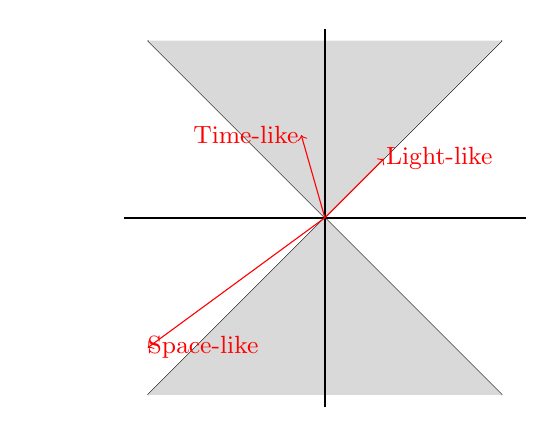
\begin{tikzpicture}[scale=1.5]
    \def\b{0.2} % semi-minor axis
    \pgfmathsetmacro{\h}{(1 + sqrt(1 + 4*\b^2)) / 2}
    \pgfmathsetmacro{\a}{sqrt(\h)}
    \draw (-1.5, -1.5) -- (1.5,  1.5);
    \draw (-1.5,  1.5) -- (1.5, -1.5);
    \fill[gray!30] (0,0) -- (1.5,1.5) -- (-1.5,1.5);
    \fill[gray!30] (0,0) -- (-1.5,-1.5) -- (1.5,-1.5);
    % \draw (0,  \h) ellipse [x radius = \a, y radius = \b];
    % \draw (0, -\h) ellipse [x radius = \a, y radius = \b];
    \draw [thick] (0,-1.6) -- (0,1.6);
    \draw [thick] (-1.7,0) -- (1.7,0);
    \draw [->, red] (0,0) -- (0.5,0.5) node {\hspace{4em}\small Light-like};
    \draw [->, red] (0,0) -- (-0.2,0.7) node {\hspace{-4em}\small Time-like};
    \draw [->, red] (0,0) -- (-1.5,-1.1) node {\hspace{4em}\small Space-like};
  \end{tikzpicture}
  \caption{The Light Cone}
\end{figure}
The gray shaded area is the accessible region of spacetime by light, the lightcone.

\subsection{Time Dilation}


